

\graphicspath{{chapters/paper3/}}


\chapter{Paper 3}
{\Huge \textbf{Efficient estimation of personalized biventricular mechanical
  function employing gradient-based optimization}}

% \clearpage
\newpage
\section*{Efficient estimation of personalized biventricular mechanical
  function employing gradient-based optimization}

% \begin{center}
  Henrik Finsberg$^{1,4,5}$,
  Ce Xi$^{2}$,
  Ju Le Tan$^3$,
  Liang Zhong$^{3,8}$,
  Martin Genet$^7$,
  Joakim Sundnes$^{1,4,5}$,
  Lik Chuan Lee$^2$, and
  Samuel Wall$^{1,4,6}$,
% \end{center}

% \onehalfspacing
\footnotesize
\begin{enumerate}[itemsep=-2mm]
\item{Simula Research Laboratory, Lysaker, Norway}
\item{Department of Mechanical Engineering, Michigan State
    University, U.S.A}
\item{National Heart Center Singapore, Singapore}
\item{Center for Cardiological Innovation, Oslo, Norway}
\item{Department of Informatics, University of Oslo, Oslo, Norway}
\item{Department of Mathematical Science and Technology, NMBU, \r{A}s,
    Norway}
\item{Mechanics Department and Solid Mechanics Laboratory, \'{E}cole
    Polytechnique, France}
\item{Duke National University of Singapore, Singapore}
\end{enumerate}
\normalsize
% \singlespace



\subsection*{Abstract}
% \abstract[Abtract]{
Individually personalized computational models of
  heart mechanics can be used to estimate important physiological and
  clinically-relevant quantities that are difficult, if not
  impossible, to directly measure in the beating heart. Here we present a novel
  and efficient framework for creating patient-specific biventricular
  models using a gradient-based data assimilation method for evaluating regional myocardial
  contractility and estimating myofiber stress. These
  simulations can be performed on a regular laptop in less than two
  hours and produce excellent fit between measured and simulated
  volume and strain data through the entire cardiac cycle. By applying
  the framework using data obtained from three healthy human
  bi-ventricles, we extracted clinically important quantities as well as
  explored the role of fiber angles on heart function. Our results
  show that steep fiber angles at the endocardium and epicardium
  are required to produced simulated motion compatible with measured strain and volume data. We also
  find that the contraction and subsequent systolic stresses in the right ventricle
  are signficantly lower than in the left ventricle. Variability of the
  estimated quantities with respect to both patient data and modeling choices are also found
  to be low. Because of its high efficiency, this framework may be
  applicable to modeling of patient specific cardiac mechanics for
  diagnostic purposes.
% }


\section{Introduction}
Cardiac computational modeling has emerged as both a powerful method to provide basic insight into cardiac function/
dysfunction, and as a support tool to improve current clinical practice. Its development
is in part driven by significant advancements in medical imaging techniques
\citep{pope2008three,townsend2008multimodality,lamata2014images}, which now provide a
wealth of information about cardiac structure and
kinematics. Merging this information with biophysical descriptions of
cardiac behavior allows for creation of powerful patient specific models
of the heart \citep{Krishnamurthy2013, Lee2014JCS, chabiniok2016multiphysics}. Such models can
 be used to predict the outcome of different treatment
strategies \citep{sermesant2012patient} or to extract
 useful indicators of mechanical function,  such as myocardial contractility
\citep{chabiniok2012estimation,finsberg2017estimating} and
myofiber stress \citep{genet2014distribution,xi2016patient}, potential biomarkers which are
currently difficult, if not impossible, to measure directly using imaging
techniques \citep{huisman1980measurement}.


Of particular importance is ventricular myofiber stress
\citep{yin1981ventricular}, which is hypothesized to be a key driver of
pathological remodeling processes in cardiac diseases
\citep{grossman1975wall}. Correspondingly, quantifying stress and determining how cardiac interventions may reduce abnormal stress is
considered a useful avenue in developing treatments for heart failure
\citep{guccione2003myosplint}. However, while measurements of heart motion
are possible using an array of imaging techniques, no direct measurements 
of the load experienced by myocytes are currently possible in vivo and 
estimates are instead used.  One widely used method is the law of Laplace, a
simplified model that takes into account pressure, wall thickness and curvature, and can guide
evaluation of stress in idealized geometries.   However, despite its wide use, it has been shown that this law severely underestimates
myofiber stress in largely irregular patient-specific ventricular geometries 
 \citep{zhang2011comparison}. Furthermore, regional stresses also
cannot be accurately estimated using this idealized law. 

In order to overcome these limitations, patient specific simulation using finite element modeling is
widely accepted as a viable way to accurately estimate myofiber
stresses in the complex geometry of the heart, and has been used in designing heart
failure treatments to reduce myocardial stress \citep{lee2013algisyl, guccione2003myosplint, Wall2006}. However, one of the many challenges faced by researchers developing patient specific models is to
efficiently and accurately incorporate individual data into the them, which often
requires determining model parameters that best reproduce the
observations i.e., data assimilation
\citep{sermesant2006cardiac,chapelle2013fundamental}.  This data assimilation usually involves
some optimization method and different techniques have been
applied to estimate these parameters in heart models. These techniques include global
methods such as parameter sweeps
\citep{asner2015estimation,Genet2015JBE} and genetic algorithms
\citep{nair2007optimizing}, as well as local methods such as gradient-based
searches \citep{balaban}.

These methods all have advantages and drawbacks.  Global methods will find the best fit in the parameter space, but typically require many functional evaluations to sweep
the entire space that can be quite costly, especially in the context of heart mechanics. Gradient-based
methods successively improve the solution by
searching along the gradient descent, and may substantially reduce the
required number of functional evaluations. However, these methods may
not find a global minimum, and in addition, estimating the
gradient by methods such as finite differences requires as
  many functional evaluations as the number of control parameters (N + 1
  evaluations for N parameters), and is therefore impractical
 if many parameters are involved.
However, new methods are emerging to solve the limitations of gradient based searches,with the automated derivation of functional gradients
via solution of the corresponding adjoint system \citep{farrell2013automated}
now offering the possibility to compute the functional gradient at a computational
expense that does not depend on the number of control parameters.

In this work, we apply such a gradient-based data assimilation framework
in order to fuse clinical imaging data from a cohort of healthy subjects to
a bi-ventricular mechanics model accurately and efficiently. By relating physical processes to the
kinematics observed in medical images, we extracted clinically
important quantities from these subject-fitted models and evaluated the
sensitivity of these quantities to modeling choices such as fiber
architecture and model for active contraction.  

The paper is organized as follows. In Section
\ref{paper3:sec:methods} we present the pipeline for data assimilation,
that includes an outline of the underlying ventricular
mechanics model and solution methods. Section \ref{paper3:sec:results}
presents the results of applying the framework to imaging data
acquired from three healthy subjects, including a comparison of model
prediction with the observed data, analysis of mechanical parameters
extracted from the model, and a sensitivity analysis of model
parameters to the input data. Finally, in sections \ref{paper3:sec:disc} and
\ref{paper3:sec:concl} we discuss the performance of the framework and draw
conclusions about its applicability in clinical settings.


\section{Methods}
\label{paper3:sec:methods}

\subsection{Data acquisition and pre-processing}

Cine magnetic resonance (MR) images of 3 healthy subjects were
acquired at the National Heart Center of Singapore and written
informed consent was obtained from all participants.
Three-dimensional biventricular geometries of each subject were
manually segmented from the MR images at multiple cardiac time points
using the medical image analysis software MeVisLab
(http://www.mevislab.de).


Cavity volumes of the left ventricle (LV) and right ventricle (RV)
were computed from the segmented geometries at different time points
in a cardiac cycle in each subject. Using a method described in
\citep{xi2016patient}, these volumes were paired with normal left and
right ventricular pressure wave forms from previous studies
\citep{Redington1988} to construct pressure-volume loops of the LV and
RV. Based on a previous empirical study \citep{Kelly1992a}, LV pressure
for each subject was also scaled so that the end-systolic pressure is
90\% of the measured cuff pressure.


Regional circumferential and longitudinal Green-Lagrange strains in
the LV free wall (LVFW), septum and RV free wall (RVFW) were estimated
in each subject using an hyperelastic warping technique \citep{Veress2005JBE, Genet20162AMISMRMI}.
Briefly, a bi-ventricular finite element model reconstructed from the end-systolic
(template) image, was registered to all other cine (target) images
acquired in the cardiac cycle by minimizing the squared difference
between the target and template image intensities. 
This ill-posed correlation problem is regularized by also minimizing a
prescribed (Neo-Hookean) strain energy function over the mesh. We note
that other regularization approaches have also been proposed, such as
regularization  based on incompressibility \citep{Mansi2011IJCV} or on equilibrium
\citep{Claire2004IJNME, Genet2017S}. Hyperelastic warping
offers a good balance between regularization and strain estimation
\citep{Genet20162AMISMRMI}. 
The implementation of the image correlation procedure is based on FEniCS
\citep{Alnaes2015}, and is freely
available\footnote{\url{https://bitbucket.org/mgenet/dolfin_dic}}.

Three-dimensional biventricular meshes of the three normal subjects were created
using Gmsh \citep{geuzaine2009gmsh} with the number of elements ranging from 4000 - 8000
tetrahedral elements. The chosen reference geometries were reconstructed
from MR images in late diastole, and all meshes were uniformly refined
in order to perform a convergence analysis .


Rule based fibers were assigned using the Laplace Dirichlet
Rule-Based (LDRB) algorithm \citep{bayer2012novel}.
Although previous histological studies \citep{streeter1969fiber}
suggest that myofiber fiber helix angle varies transmurally from
$+60^{\circ}$ at the endocardium to $-60^{\circ}$ at the epicardium,
variability in fiber angle,  nevertheless, exists between individuals.
Therefore, we seek to also test how different fiber angle gradient
alters the parameter estimation and the extracted outputs.
More specifically, an angle $+\alpha/-\alpha$ is prescribed on the
endo-/epicardium for $\alpha$ ranging from $30^{\circ}$ to $80^{\circ}$ at
increments of  $10^{\circ}$. If not otherwise specified, an angle of $+60^{\circ}$ and
$-60^{\circ}$ on the endo- and epicardium respectively is prescribed. In
Figure \ref{paper3:fig:fiber_angles} we show this range of fiber fields for
one of the subjects.


\begin{figure}[htbp]
    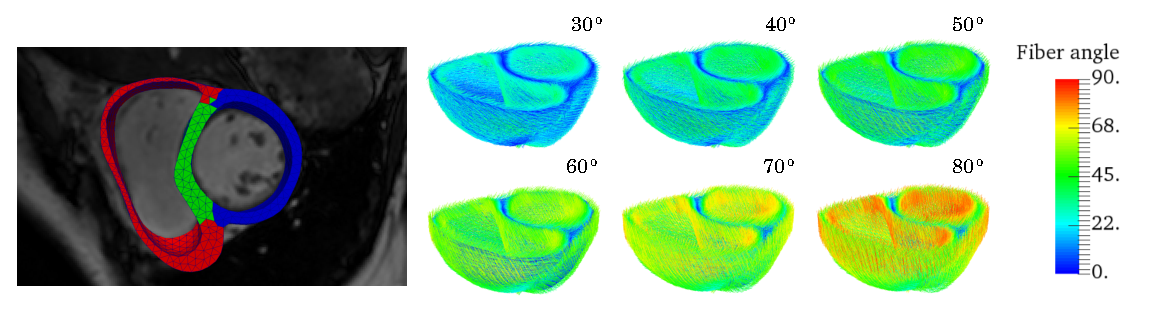
\includegraphics[width=\textwidth]{figures/fiber/fiber_v2}
\caption{\label{paper3:fig:fiber_angles} Left: finite
    element mesh of a biventricular geometry reconstructed from MR
    images separated into 3 material regions, namely, LVFW (blue),
    septum (green) and RVFW (right). Right: myocardial fiber
  orientation are assigned using the LDRB algorithm
  \citep{bayer2012novel} with an angle $+\alpha$ and 
  $-\alpha$ prescribed on the endocardium and epicardium, respectively. Here
  showing the fiber architecture for $\alpha$ ranging from
  $30^{\circ}$ to $80^{\circ}$ with increments of $10^{\circ}$, where
  the absolute value of the fiber angle is used as
  color-map.} 
\end{figure}





\subsection{Mechanical modeling}
\label{paper3:sec:mechanical_model}

We consider a configuration of a biventricular continuum body
$\mathfrak{B}$, which is a function $\kappa : \mathfrak{B} \rightarrow
\mathbb{R}^3$, and denote the reference and current configurations
by $\Omega_0 = \kappa_0 (\mathfrak{B}) $ and $\Omega = \kappa
(\mathfrak{B}) $, respectively. Letting $\Xvec$ and $\xvec$
be the coordinates of a given material point in the reference and
current configuration respectively, we have the corresponding
displacement field $\uvec = \xvec-\Xvec$, and the deformation gradient 
\begin{align}
  \F = \frac{\partial \uvec}{\partial \Xvec} + \I.
\end{align}
Mechanics of the heart wall was described using an active strain
formulation \citep{ambrosi2011electromechanical} that assumes a
multiplicative decomposition of the deformation gradient,
\begin{equation}
 \F = \F_e \F_a.
\label{paper3:eq:active_strain}
\end{equation}
Here, $\F_a$ is associated with an inelastic deformation resulting from the
actively contracting muscle fibers, whereas $\F_e = \F \F_a^{-1}$ is
associated with the elastic deformation that preserves compatibility
in the tissue, and passively carrying the mechanical load. We choose
$\F_a$ to have the specific form  
\begin{equation}
  \F_a = (1 - \gamma) \ef \otimes \ef  + \frac{1}{\sqrt{1 - \gamma}} (\I - \ef \otimes \ef),
 \label{paper3:eq:active_strain_Fa_gjerald}
\end{equation}
in which the parameter $\gamma$ is associated with the relative active
shortening along the muscle fibers. The same form of the active
deformation gradient has previously been applied in e.g
\citep{gjerald2014patient,balaban}.


We consider the transversely Holzapfel and Ogden hyperelastic material
\citep{holzapfel2009constitutive} model that has the strain energy
density function
\begin{align}
\label{paper3:eq:holzapfel_ogden}
\Psi(\F) = \frac{a}{2 b} \left( e^{ b (I_1  - 3)}  -1 \right)
 + \frac{a_f}{2 b_f} \left( e^{ b_f (I_{4\ef} - 1)_+^2} -1 \right),
\end{align}
where the invariants are given by
\begin{align}
  I_1 = \tr \C, \;\; I_{4\ef} = \ef \cdot (\C \ef).
\end{align}
Here $\C = \F^T\F$ is the right Cauchy Green tensor, and $\ef$ denotes
the unit fiber field in the reference configuration.
Within the active strain formulation, the strain energy depends only on
elastic deformations, and so the modified strain energy function
$\Psi = \tilde{\Psi}(\F_e)$ was used instead. 

For comparison, we also test the more frequently used active stress
formulation \citep{hunter1998modelling}. In this formulation, the total Cauchy
stress tensor is additively decomposed into a passive and an active component i.e.,
\begin{align}
  \Cauchy = \Cauchy_p + \Cauchy_a,
\end{align}
where the passive stress tensor is given by
\begin{align}
  \Cauchy_p = \frac{1}{J} \frac{\partial \Psi}{\partial \F}\F^T,
\end{align}
and the active stress tensor is given by
\begin{align}
  \Cauchy_a = T_a \left[\Fef \otimes \Fef +
   \eta\left(\I - \Fef \otimes \Fef \right)\right].
  \label{paper3:eq:active_stress}
\end{align}
Here $T_a$ is the magnitude of the active stress and $\eta$ controls
the amount of transverse active stresses.
Although active stresses, in principle, develop along the fiber
direction, studies have shown \citep{lin1998multiaxial} that active
stresses in the transverse direction are non-negligible due to
imperfect alignment of the muscle fibers. We therefore set $\eta =
0.2$ \citep{sundnes2014improved}, and note that transverse active
stresses are naturally embedded in the active strain formulation by
requiring $\mathrm{det}\;\F_a = 1$ .

Myocardium was assumed to be incompressible. The incompressibility was
enforced in the model using a two-field variational approach, in which
the term $-p(J-1)$ was added to the total strain energy with $p$
denoting a Lagrange multiplier that represents the hydrostatic
pressure. The deviatoric and volumetric mechanical responses were also
uncoupled by multiplicatively decomposing the deformation gradient
\citep{weiss1996finite}, 
\begin{align}
  \F = \F_{\mathrm{iso}}\F_{\mathrm{vol}}
  \label{paper3:eq:deviatoric_split}
\end{align}
and letting the strain-energy be a function of only isochoric
deformations i.e., $\Psi = \bar{\Psi}(\F_{\mathrm{iso}})$.
  
Ventricular base was fixed in the longitudinal direction and the
biventricular geometry was anchored by constraining the
epicardial surface using a Robin-type boundary condition with a linear
spring of stiffness $k=0.5$ kPa/cm$^2$ \citep{xi2016patient}.
Measured cavity pressure in the LV ($\plv$) and RV ($\prv$) were
applied as a Neumann condition at the endocardial surfaces.
The Euler-Lagrange equations in the Lagrangian form reads: Find
$(\uvec, p) \in V \times Q$ such that for all $ (\delta \uvec, \delta
p) \in V \times Q$ and $\left. \left( \uvec \cdot \N \right)
\right|_{\partial \Omega_0^{\mathrm{base}}} = 0$ ,

\begin{align}
  \delta\Pi(\uvec, p) &=
  \int_{\Omega_0} \left[ \FPiola: \nabla \delta \uvec  - \delta p (J - 1 ) - pJ\F^{-T}:\nabla \delta \uvec \right] \mathrm{d}V
  + \delta\Pi_{\text{ext}} = 0,
  \label{paper3:eq:force_balance}
\end{align}
with
\begin{align}
  \begin{split}
  \delta \Pi_{\text{ext}} &=
  \int_{\partial \Omega_0^{\mathrm{endo} \; \mathrm{LV}}} \plv J \F^{-T} \N \cdot \delta \uvec \mathrm{d}S \\ &+
  \int_{\partial \Omega_0^{\mathrm{endo} \; \mathrm{RV}}} \prv J \F^{-T} \N \cdot \delta \uvec \mathrm{d}S +
  \int_{\partial \Omega_0^{\mathrm{epi}}} k \uvec \cdot \delta \uvec \mathrm{d}S.
 \end{split}
  \label{paper3:eq:bndry_cond}
\end{align}

\noindent
Here $V = H^1(\Omega_0)$, completed with homogeneous Dirichlet boundary
data, $Q = L^2(\Omega_0)$, $ \N $ is the outward pointing unit normal
and  $\FPiola$ is the first Piola-Kirchhoff stress tensor.

\subsection{PDE-constrained optimization}
The ventricular mechanics model outlined in Section \ref{paper3:sec:mechanical_model}
contains model parameters that may vary from individual to
individual.
Calibration of these model (or control) parameters was achieved by solving a
PDE-constrained optimization problem, where we minimized a cost functional
representing the mismatch between the simulated and
observed data, subject to the constraint of satisfying
\eqref{paper3:eq:force_balance}-\eqref{paper3:eq:bndry_cond}.
The minimization problem can be formally stated as
\begin{equation}
  \begin{aligned}
    \label{paper3:eq:optimization_problem}
    & \underset{m}{\text{minimize}}
    & &  \mathcal{J}((\uvec, p), m) \\
    & \text{subject to}
    & & \delta \Pi(\uvec, p) = 0.
  \end{aligned}
\end{equation}
Here $\mathcal{J}$ is the objective functional that we want to
minimize, which depends on the state variable $(\uvec, p)$ and the
control parameter(s) $m$. The state variables may also depend on the
control parameters $(\uvec, p) = (\uvec(m), p(m))$. To ease
notation, this dependency is not explicitly stated here.

Minimization of the cost functional $\mathcal{J}$, should bring
the simulated results closer to the clinical observations. Therefore,
$\mathcal{J}$ should reflect a distance between the model and the data.  
Given a measurement point $i$, let $(\uvec^i,p^i)$ be the simulated state
variables at that point, and let $m^i$ represents any generic model
parameter, that we want to estimate. The cost functional is then
given by
\begin{equation}
  \mathcal{J}((\uvec^i,p^i), m^i)
  = \alpha \mathcal{J}_{\mathrm{volume}}((\uvec^i, p^i), m^i)
  + \beta \mathcal{J}_{\mathrm{strain}}((\uvec^i, p^i), m^i)
  + \lambda \mathcal{J}_{\mathrm{reg}}(m^i).
  \label{paper3:eq:total_functional}
\end{equation}
The first two terms represent the mismatch between simulated and
observed strains and volumes, whereas $\mathcal{J}_{\mathrm{reg}} $ is
a regularization term that penalizes non-smooth values of the control
parameter $m^i$ for numerical stability. The weights $\alpha, \beta$
and $\lambda$ control what terms is favored in the optimization.


The cavity volume was given by
\begin{equation}
  \tilde{V}_{\cdot} = - \frac{1}{3} \int_{\partial \Omega_0^{\mathrm{endo}\; \cdot}} (\Xvec + \uvec )J \F^{-T} \N \mathrm{d} S.
\end{equation}
This equation holds as long as the base remains flat and is located at the $x=
0$ plane. We let $\mathcal{J}_{\mathrm{volume}}$ be the sum of the
squared relative volume error in each chamber:
\begin{equation}
  \mathcal{J}_{\mathrm{volume}}((\uvec^i, p^i), m^i) =
  \left( \frac{V_{\text{LV}}^i - \tilde{V}_{\text{LV}}^i}{V_{\text{LV}}^i} \right)^2
  + \left( \frac{V_{\text{RV}}^i- \tilde{V}_{\text{RV}}^i}{V_{\text{RV}}^i} \right)^2.
  \label{paper3:eq:I_vol}
\end{equation}
Here, $(\tilde{V}_{\text{LV}}, \tilde{V}_{\text{RV}})$ and
$(V_{\text{LV}}, V_{\text{RV}}) $ are the simulated and measured
cavity volumes, respectively.

Volumetric averaged strains were computed in each material region
(i.e., LVFW, RVFW and septum) using end-diastole (ED) as
reference. Letting $\F_{\mathrm{ED}}$ be the deformation gradient
tensor associated with ED, the Green-Lagrange strain tensor with ED as
reference was given by $\tilde{\mathbf{E}} =
\frac{1}{2}(\F^T\F_{\mathrm{ED}}^{-T} \F\F_{\mathrm{ED}}^{-1} -\I)$.
Normal averaged strain along the circumferential direction
$\mathbf{e}_{\mathrm{circ}}$ in material region $\Omega_j$ was 
defined by 
\begin{align}
   \tilde{\varepsilon}_{j} = \frac{1}{|\Omega_j|}
   \int_{\Omega_j}\mathbf{e}_{\mathrm{circ}} \cdot \tilde{\mathbf{E}} \mathbf{e}_{\mathrm{circ}} \mathrm{d} V .
\end{align}
Correspondingly, the strain mismatch functional was given by the total
squared error between the simulated circumferential strain
$\tilde{\varepsilon}_{j}^i$ and the measured circumferential strain
$\varepsilon_{j}^i$ over all material regions 
\begin{equation}
  \mathcal{J}_{\mathrm{strain}}((\uvec^i, p^i), m^i)  =\sum_{j= 1}^{N} \left( \varepsilon_{j}^i -  \tilde{\varepsilon}_{j}^i \right)^2.
  \label{paper3:eq:I_strain}
\end{equation}
Finally, the regularization term was defined as the total squared distance
from the mean value, that is if $m^i = (m_1, \cdots, m_N)$, then
\begin{align}
\mathcal{J}_{\mathrm{reg}}(m^i) = \sum_{j=1}^{N} (m_j^i - \overline{m}^i )^2 , &&  \overline{m}^i = \frac{1}{N} \sum_{j=1}^{N} m_j^i.
\end{align}
As noted above, the purpose of this term is to avoid numerical
instabilities by penalizing large variations in the control parameters.




\subsection{Parameter estimation}
The pipeline for fitting the model to patient data was 
divided into two sequential phases; a passive phase where we estimated the
material parameters that define the passive behavior of the
myocardium, and an active phase where we estimated the amount
of active contraction.
In both cases, the control parameters were 
spatially resolved. During the passive phase the control parameter was
allowed to vary spatially on the LV (LVFW+septum) and RV segments, while in the active
phase the LV was separated into LV free wall and septal segments, which provided
additional degree of freedom to allow for non-homogeneous LV contraction.


Geometries used in the simulation were reconstructed from medical
images. These geometries are, in principle, not load-free. Hence, we
need to estimate the unloaded (zero pressure) geometries, which  will
revert  back to the original reconstructed geometries when loaded with
the measured pressure. Several methods exists for estimating the
unloaded geometry \citep{govindjee1996computational,gee2010computational}. 
Among the most simplest ones is the backward displacement method
\citep{sellier2011JFS,bols2013computational} that can also be used to
incorporate residual stresses into the finite element models by
simulating tissue growth \citep{Genet2015JB}. Nevertheless, this
inverse problem (of finding the unloaded geometry) has  been shown to
produce non-unique solutions, especially when buckling is present
\citep{govindjee1996computational}, although relaxation techniques can
be used to improve convergence and stability \citep{Rausch2017JB}. For
the case of a bi-ventricular geometry, buckling may occur due to the
thin RVFW and a high RV pressure. For this reason, we choose a simpler
approach to estimate  the unloaded configuration. As shown in the left
of Figure \ref{paper3:fig:pipeline}, we start by applying one iteration of
the backward displacement method with initial values prescribed for
the material parameters followed by the material parameter estimation
as outlined below. This will result in a deflated geometry as shown in
the right of Figure \ref{paper3:fig:pipeline}. A sensitivity analysis
(\ref{paper3:sec:unloaded_sens}) was conducted to assess how the choice of
the initial material parameter values affects our results. 


Four material parameters i.e., $a$, $a_f$, $b$ and $b_f$
\eqref{paper3:eq:holzapfel_ogden} have to be estimated in the passive phase.
Due to the sparsity of passive data used for the optimization, if we
let all these parameters vary freely, we may end up in a situation
where multiple parameter sets will equally minimize the cost functional, and the
optimal control will depend heavily on the initial guess of the optimization.
We therefore restricted our control parameter to be only the linear
isotropic parameter with an initial guess $a=1.291$kPa, and have the
remaining parameters fixed according to \citep[Table 2, case
P2]{asner2015estimation}. The weights were set $\alpha = 1.0, \beta =
0.0$ and $\lambda = 10^{-6}$ in \eqref{paper3:eq:total_functional} so that
only ED volumes were used for fitting.  
Since fitting the left and right ventricular
end diastolic volumes might require different material
properties of the left and right ventricular wall, the parameter $a$ was
spatially resolved with one parameter associated with the LV (LVFW +
septum) and one parameter associated with the RVFW


In the active phase, the optimized material parameters were fixed and
the relative active fiber shortening $\gamma$ in
\eqref{paper3:eq:active_strain_Fa_gjerald} was chosen as control
parameter. For this phase, the weights in \eqref{paper3:eq:total_functional}
were set to $\alpha = 0.1,  \beta = 1.0$ and $\lambda = 10^{-4}$, so
that both strain and volume are considered in the optimization. This
choice of weighting was made ad hoc, reflecting the relative size of
the different terms in the cost functional. It should also be noted
that the volume functional in \eqref{paper3:eq:I_vol} is a relative error
while the strain functional in \eqref{paper3:eq:I_strain} represents a total
error. 

For each time point, we estimated $\gamma$ locally in the LVFW, RVFW
and septum. The initial guesses for the optimization were set to zero
in the first iteration. In subsequent iterations, the initial guesses
were set to the optimized values found in the previous iteration.
Note that in the case when active stress formulation was used instead,
the parameter $T_a$ in \eqref{paper3:eq:active_stress} was used as the
control parameter and estimated in a similar fashion. 

A schematic illustration of the full optimization pipeline is provided
to the left in Figure \ref{paper3:fig:pipeline}.

\begin{figure}[htbp]
  \centering
  \includegraphics[width=\textwidth]{figures/models}
  \caption{\label{paper3:fig:pipeline}To the left we see the
    model-personalization pipeline. The image-based
    geometry corresponds to some image frame taken at mid diastole. An
    estimate of the unloaded geometry was found by applying one
    iteration of the backward displacement method using $a = 1.291$ kPa
    according to \citep{asner2015estimation}, followed by an estimation
    of $a$ by minimizing the fit of the end-diastolic volumes. During
    systole, both cavity volumes and circumferential strain were used in
    the optimization to determine the amount of active contraction in
    terms of the active control, which are respectively  $\gamma$ and $
    T_a$ in the active strain and active stress formulation. To the
    right we show a comparison of the unloaded geometry for CASE3. The
    upper figure shows the resulting unloaded, zero pressure geometry in
    red and the the original image-based geometry in transparent, while
    the bottom figure shows the unloaded geometry, inflated to the target
    pressure in the image-based geometry, and the original image-based
    geometry in transparent for comparison.}
\end{figure}

\subsection{Mechanical Analysis}

%\subsubsection{Stress analysis}
% Abnormalities in ventricular wall stress is believed to be responsible
% remodeling processes associated with heart failure. It is therefore of
% interest to compute the stresses in the personalized simulations.
For an incompressible, hyperelastic, continuum body, the total Cauchy
stress tensor is given by
\begin{align}
  \Cauchy = \frac{1}{J} \frac{\partial \Psi(\F)}{\partial \F} \F^T - p\I.
  \label{paper3:eq:total_cauchy_stress}
\end{align}
With the decoupling of the isochoric and volumetric deformation
according to \eqref{paper3:eq:deviatoric_split},
the first term in \eqref{paper3:eq:total_cauchy_stress} represents the
deviatoric stresses and $p$ is the hydrostatic pressure. Myofiber
stress was computed by first a push forward of the fiber field to the current
configuration, $\mathbf{f} = \F \mathbf{f}_0$, and then an inner
product with the stress tensor $\Cauchy_{\mathbf{f}} = \mathbf{f}
\cdot \Cauchy \mathbf{f}$. The average fiber stress in a given region
$\Omega_j$ was computed by integrating the fiber stress over that
region and dividing by the volume i.e.,
$\overline{\Cauchy_{\mathbf{f}}}^{\Omega_j} = | \Omega_j |^{-1}
\int_{\Omega_j} \Cauchy_{\mathbf{f}} \mathrm{d} V$.

%\subsubsection{Contraction analysis}
The control parameter in the active phase represents an index of
contractility \citep{finsberg2017estimating}, meaning that the higher
the value of the control parameter, the more forcefully the myocardium is
trying to contract against the external loads. To separate between the LV and
RV contractility, we extracted the average value of this control parameter in these
two segments. Another index of contractility is the end systolic
elastance \citep{sagawa1977end}, which we have also estimated in the LV and
RV by perturbing the loading conditions at the end systolic state and
estimate the slope of the resulting pressure-volume
relationship \citep{finsberg2017estimating}.


\subsection{Implementation details}
The force-balance equations were solved using the finite element
method, whereby the displacement and hydrostatic pressure fields were
interpolated using piecewise quadratic and linear basis functions,
respectively. These mixed elements, known as the Taylor-Hood finite
elements \citep{hood1974navier}, are known to satisfy the discrete
inf-sup condition \citep{chapelle1993inf} and leads to a stable
discretization. The solver was implemented in FEniCS
\citep{logg2012automated}, which is an open-source platform for
solving PDEs using the finite element method. Nonlinear systems of
equations were solved using Newton's method,
and a distributed memory parallel LU solver\citep{li2003superlu_dist}
was used to solve the linear systems.


To solve the optimization problem \eqref{paper3:eq:optimization_problem} we
applied a sequential quadratic programming algorithm (SQP)
\citep{kraft1988software}. This gradient-based optimization
algorithm requires the functional gradient, that is the derivative
of the functional $\mathcal{J}$ in \eqref{paper3:eq:total_functional}, with
respect to the control parameters. This gradient was
computed by solving an automatically derived adjoint equation using
dolfin-adjoint \citep{farrell2013automated}.
The full source code is publicly
  available\footnote{\url{https://bitbucket.org/finsberg/pulse_adjoint}}. 

\section{Results}
\label{paper3:sec:results}
In this section we present the results from the model personalization
process. Results of the data matching are 
presented in Section \ref{paper3:sec:data_asssim}, together with a validation of the
model and analysis of the solver performance. To validate the model we compare the
simulated and measured longitudinal strain which was not used in the
optimization. In Section \ref{paper3:sec:mech_analysis} we present the results of the
extracted mechanical features such as indices of contractility and
fiber stress.  We also investigated the efficiency of the algorithm and the effect of mesh refinement, and
found that the chosen refinement level was sufficient to yield
convergent solutions.

\subsection{Data assimilation, validation and solver performance}
\label{paper3:sec:data_asssim}
\label{paper3:sec:validation}
\label{paper3:sec:sys_perform}
%The simulated pressure-volume (PV) loops of LV and RV were in close
%agreement with the measured PV loops, as shown in the left panel of Figure
%\ref{paper3:fig:data_matching}. 
The simulated and measured pressure-volume (PV) loops of the RV and LV, as well as circumferential strain in the LV, septum
and RV are shown in Figure \ref{paper3:fig:data_matching}. We found that the fit of the data was highly dependent
on the choice of fiber angles, which affects both volume change and circumferential shortening. Plotting the average value of the
volume cost functional (as defined in \eqref{paper3:eq:I_vol}) for each
choice of fiber angles as shown in the upper right panel in
Figure~\ref{paper3:fig:data_matching}, revealed that the optimal value of
$\alpha$ lies in the range $70^{\circ}-80^{\circ}$ for all 3 cases.


\begin{figure}[htbp]
 \centering
  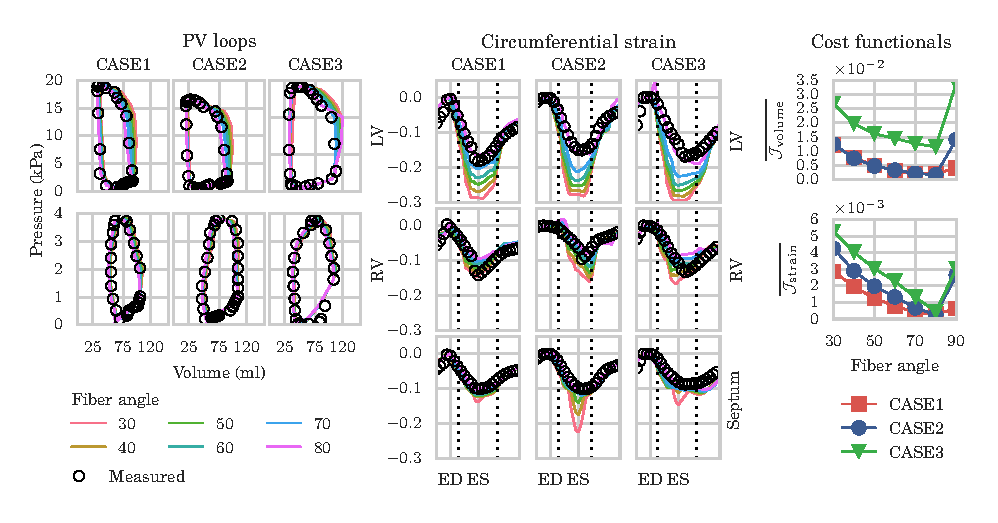
\includegraphics[width=\textwidth]{figures/data_matching}
  \caption{\label{paper3:fig:data_matching}Results of the gradient-based
    minimization of model-data mismatch for different choice of fiber
    angles. Left: simulated (color lines) and measured (black circles)
    PV loops in the LV (top row) and RV (bottom row). Center:
    simulated (color lines) and measured (black circles)
    circumferential strain in the LV (top row), RV (middle row ) and
    septum (bottom row). Right: average values of cost functional for
    the volume (top row) and strain (bottom row), for each choice of
    fiber angle.}  
\end{figure}


Although available, we chose not to use longitudinal strain data in the
optimization. Therefore, the comparison of model-predicted
longitudinal strain with the measurements serves as a validation of the
model-personalization process. The simulated and measured LV
longitudinal strain curves are shown in Figure
\ref{paper3:fig:fiber_long}. We note that the fit in all regions was again highly sensitive
to the choice of fiber angle. Choosing $\alpha = 70^{\circ}$ produced the best
fit for the LV longitudinal strain for CASE1 and CASE3, while an angle
$60^{\circ}$ gave the best fit for CASE2. The Septal and RV
longitudinal strain was best fitted with $\alpha = 80^{\circ}$.  


\begin{figure}[htbp]
 \centering
  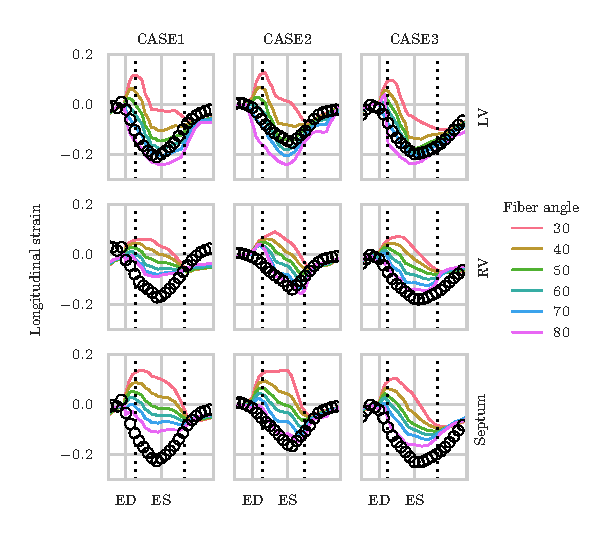
\includegraphics[width=\textwidth]{figures/longitudinal_strain}
  \caption{\label{paper3:fig:fiber_long}Validation of the
    model-personalization process using simulated and measured
  longitudinal strain which was not used in the optimization. Upper,
  middle and lower panel show the longitudinal strain
  curves for different choice of fiber angles in the LV, RV and septum respectively.}
\end{figure}

% \subsection{Solver performance}
We further evaluated the solver performance in the optimization process.  In this work, all computations were performed on a computing cluster using one node
with 8 cores. In Table \ref{paper3:tab:timings} we present timings for evaluation of
the forward model (i.e., evaluation of the cost functional), timings for
evaluation of the gradient, as well as the average number of such
evaluations and the standard deviations. These timings are shown for
optimizations using the original and refined meshes with a fiber
angle of $60^{\circ}$. 


\begin{sidewaystable}
\caption{Timings for evaluation (eval) of the forward model and the gradient,
  running on one computing node with 8 cores for the different subjects
  with different mesh resolutions. The average number of forward
 and gradient evaluations for each measurement points are also shown
 along with the standard deviations.}
\begin{tabular}{lllllll}
\toprule
  Patient ID   & $\#$ elements   & forward eval time (s)
  & $\#$ forward eval   & gradient eval time (s)
  & $\#$ gradient eval & Total run time (h)  \\
  \midrule
  \multirow{2}{*}{CASE1}
               &7362  & 32 $\pm$ 19.8   & 9 $\pm$ 1.6  & 9 $\pm$ 0.1  & 8 $\pm$ 1.5 & 1.97\\
               &58896 & 668 $\pm$ 529.8 & 9 $\pm$ 1.7  & 81 $\pm$ 1.3 & 7 $\pm$ 1.6 & 36.1\\
  \hline
  \multirow{2}{*}{CASE2}
               & 4755  & 19 $\pm$ 9.6    & 9 $\pm$ 2.1  & 8 $\pm$ 0.1  & 8 $\pm$ 2.0 & 1.88\\
               & 38040 & 387 $\pm$ 325.8 & 9 $\pm$ 2.5  & 47 $\pm$ 0.4 & 8 $\pm$ 2.2 & 32.6\\
  \hline
  \multirow{2}{*}{CASE3}
               & 4377  & 17 $\pm$ 5.3    & 10 $\pm$ 2.1 & 8 $\pm$ 0.9  & 8 $\pm$ 2.1 & 1.35\\
               & 35016 & 259 $\pm$ 146.3 & 9 $\pm$ 2.4  & 42 $\pm$ 0.7 & 8 $\pm$ 2.2 & 15.6\\
\bottomrule
\end{tabular}
\label{paper3:tab:timings}
\end{sidewaystable}



\subsection{Mechanical analysis}
\label{paper3:sec:mech_analysis}
\subsubsection{Cardiac contraction}
The estimated active strain parameter $\gamma$ in
\eqref{paper3:eq:active_strain_Fa_gjerald}, which served as the control parameter
during the optimization in the  active phase, is plotted for various fiber angles to the
left in Figure \ref{paper3:fig:mechanical_analysis}. This parameter
varies regionally in the LVFW, septum and RVFW, but is shown here as
an average in the LV containing LVFW + septum (top) and RV containing
only RVFW (bottom). As shown in the figure, time-variation and
magnitude of $\gamma$ were similar in the 3 cases and insensitive to
the prescribed fiber angles. 

\begin{figure}[htbp]
  \centering
  \includegraphics[width=\textwidth]{figures/mechanical_analysis}
  \caption{\label{paper3:fig:mechanical_analysis}To the left, average traces of the active strain
    parameter $\gamma$ in \eqref{paper3:eq:active_strain_Fa_gjerald} in the
    LV (top) and RV (bottom) for different choice of fiber angle. To
    the right average traces of Cauchy fiber stress in the  LV (top)
    and RV (bottom) for different choice of fiber angle. The
    fiber angles were defined symmetrically across the wall with a
    negative angle on the epicardium and a positive angle on the
    endocardium ranging from $30^{\circ} - 80^{\circ}$ with increments
  of $10^{\circ}$. On the $x-$axis we plot the normalized time with
  respect to end-diastole (ED) and end-systole (ES). Horizontal dotted
lines indicate timings of opening of the aortic and mitral valve.}
\end{figure}

Time traces of the active strain parameter $\gamma$ found in the LV
and RV are plotted together for the $60^\circ$ fiber angle case in the
left of Figure \ref{paper3:fig:active_stress_conv} in order better compare
their differences. A similar plot of the active stress parameter $T_a$
in logarithmic scale is also shown in the same figure. As shown in
the figure, the time-variations of $T_a$ and $\gamma$, which are
indices of cardiac contractility, were largely similar between the LV
and RV with peak values located approximately at end-systole. Peak
values found in the RV were, however, lower than those found in the
LV. These findings were consistent across all the 3 cases.

\begin{figure}[htbp]
  \centering
  \includegraphics{figures/mechanics_mesh_conv}
  \caption{\label{paper3:fig:active_stress_conv}Comparison of fiber stress
    and cardiac contraction using the active strain and active stress
    approach using $60^{\circ}$ fiber angle.
    To the left, average traces of the active stress (top) parameter $T_a$
    in \eqref{paper3:eq:active_stress}, and the active strain (bottom)
    parameter in \ref{paper3:eq:active_strain_Fa_gjerald}.  The active
    stress parameter, with unit kPa, is plotted on a logarithmic scale
    for easier comparison with the active strain parameter.
    To the right, estimated
    Cauchy fiber stress using the active
    stress (top) and active strain formulation (bottom).  On the $x-$axis we
    plot the normalized time with respect to end-diastole (ED) and
    end-systole (ES). Horizontal dotted lines indicate timings of
    opening and closing of the aortic valve.}
\end{figure}


\subsubsection{Fiber stress}
Time traces of the average Cauchy fiber stress are shown on the right
of Figure \ref{paper3:fig:mechanical_analysis} for different fiber angle
variations.  Only very small variations in the average fiber stress
were found with respect to the choice of fiber angle in the
optimization process. Snap shots of the fiber stress distribution at
ED and ES are plotted in Figure \ref{paper3:fig:mesh_res_stress_snapshots}
for the  $60^{\circ}$ fiber angle case. Regional variation of fiber
stress was largely consistent between the 3 cases with pockets of high
and low stresses found, respectively, at the apex-epicardial and
endocardial regions at ES.

In Figure \ref{paper3:fig:active_stress_conv}, we compare the average fiber stress
time variation found using the two different active contraction
formulations, either active strain or active stress. As shown in the figure, fiber stress computed using
active stress and active strain formulations behaved similarly with
time. Similar regional variation was also found where both
formulations predicted higher fiber stress in the LV than 
the RV. Peak fiber stress predicted in the LV, however, was different in
the two formulations with higher stress occurring at isovolumic
relaxation in the active stress formulation. 

\begin{figure}[htbp]
  \centering
  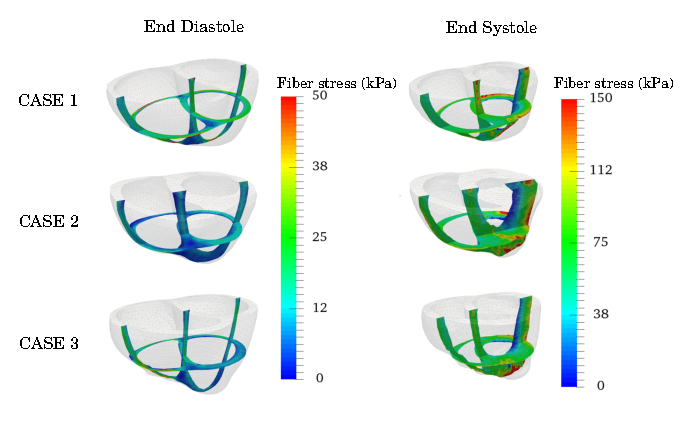
\includegraphics{figures/snapshots/stress}
  \caption{\label{paper3:fig:mesh_res_stress_snapshots}Snap shots of the end
    diastolic and end systolic configuration and the estimated fiber
    stresses shown as color-map.}
\end{figure}


The specific average value of the end-diastolic and end systolic fiber
stress for the case of a $60^{\circ}$ fiber angle are displayed in
Table \ref{paper3:tab:fiber_stress}, showing small variability between patients, despite differences in
individual PV loops.  

\begin{table}
  \centering
\caption{Average LV and RV fiber stress and end diastole and end systole}
\begin{tabular}{lrrrr}
\toprule
  Patient ID   &   LV (ED) &   RV (ED) &   LV (ES) &   RV (ES) \\
  \midrule
  CASE1        &      5.76 &      4.87 &      48.3 &      19.2 \\
  CASE2        &      4.04 &      3.57 &      54.4 &      22.7 \\
  CASE3        &      9.94 &      8.34 &      40.3 &      18.2 \\
  \hline
  Average $\pm$ std & 6.58 $\pm$ 2.48 & 5.59 $\pm$ 2.01 & 47.65 $\pm$ 5.74 & 20.03 $\pm$ 1.91 \\
\bottomrule
\end{tabular}
\label{paper3:tab:fiber_stress}
\end{table}


\subsubsection{Ventricular Elastance}

Table \ref{paper3:tab:elastance} shows the estimates of ES elastance in the
LV and RV that were computed using the active strain formulation. 
The table shows the average $\pm$ one standard deviation of the ES
elastance over various fiber angles. Elastance was consistently
found to be $\sim 10$ times larger in the LV than in the RV, and was 
largely insensitive to the prescribed fiber angle as indicated by the
small standard deviation.  

\begin{table}
  \centering
\caption{LV and RV end-systolic elastances estimated
  by perturbation of model at the end-systolic state. Average values and
  standard deviation with respect to varying fiber angle are shown.}
\begin{tabular}{lll}
\toprule
 Patient ID   & LV (kPa/ml)     & RV (kPa/ml)     \\
\midrule
 CASE1        & 1.96 $\pm$ 0.06 & 0.23 $\pm$ 0.02 \\
 CASE2        & 1.94 $\pm$ 0.14 & 0.18 $\pm$ 0.01 \\
 CASE3        & 1.52 $\pm$ 0.07 & 0.21 $\pm$ 0.01 \\
\bottomrule
\end{tabular}
\label{paper3:tab:elastance}
\end{table}


\section{Discussion}
\label{paper3:sec:disc}
In this study, we have presented a novel and highly efficient method for non invasive
personalization of an image-based bi-ventricular mechanics model based
on regional measurements of circumferential strain, as well as global
measurements of volumes and pressures in the LV and RV.
A gradient based optimization method was used to
minimize the model-data mismatch by solving a PDE-constrained optimization problem for
each measurement point in order to calibrate model
parameters. Passive material parameters and an unloaded
(zero-pressure) geometry were estimated using the bi-ventricular
geometry that was reconstructed from MR images acquired at late
diastole. Time variation of an active contraction parameter was
estimated throughout the cardiac cycle starting from ED. 

This framework was applied using measurements from three normal subjects to
extract estimates of regional fiber stress as well as indices of myocardial
contractility.  Sensitivity analysis of the model outputs with respect
to the choice of fiber angle distribution, mesh resolution and active
formulation were also conducted. The described framework is
effective and efficient in capturing cardiac mechanical behavior
throughout the cardiac cycle, and gave low patient-to-patient variabililty in the extracted mechanical features.  As such, it has potential clinical utility in
the quantification of contractile function and myocardial stress
{\it in vivo} and the potential differentiation of pathological states.



\subsection{Data compatibility and multi-objective optimization}

The objective functional in  problem \eqref{paper3:eq:optimization_problem}
consists of a weighted sum of different objective functionals.
Such problems are referred to as multi-objective optimization problems
\citep{marler2004survey}.  While it is possible to perfectly match the
strain or volume data individually with the chosen control parameters (data not shown), there is
expected to be a trade-off when fitting both the volume and strain data
 in a combined objective functional. In such
cases, a single, unique optimum does not always exist, but rather
a family of so called Pareto optimal solutions can be found \citep{marler2004survey}.
The particular solution found will depend on the chosen weights of
each objective.

In a previous study \citep{balaban}, the weights in the total
functional given in \eqref{paper3:eq:total_functional} were determined by performing an
exhaustive search, testing several combinations of weights of the strain and volume
functionals, and choosing the corner-point of strain versus volume
error curve. However, the weights will depend on the data 
source, and in our case choosing the weights proposed in \citep{balaban},
resulted in an excellent fit of the volume, while a relatively
poor fit of the strain, and hence a higher weight was chosen for the
strain. Nevertheless, neither was captured exactly, and which data
source is more important for model utility remains to be
determined. In addition, other general methods for solving
multi-objective optimization problems \citep{marler2004survey} may be
superior to the weighted sum method used here, and will be considered
in future studies. 

\subsection{Fiber angle sensitivity}
In this work, we applied a rule-based algorithm \citep{bayer2012novel} to
assign myocardial fiber orientations to the bi-ventricular geometries,
and investigated the sensitivity of the data matching and the extracted
mechanical features to the choice of fiber field.
Different fiber fields, in which the fiber angle varies linearly
across the myocardium wall from $\alpha$ at the endocardium to
$-\alpha$ at the epicardium were tested, for the range $30^\circ \leq \alpha \leq
80^\circ$. Our results show that $\alpha$ has to be in the upper part
of the range i.e., $70-80^{\circ}$, in order to fit the PV loop and
circumferential strain measurements simultaneously.
The validation study (Section \ref{paper3:sec:validation}), where we compared
our model results with the longitudinal strain, confirms this finding. 

This highlights a major challenge in building accurate mechanics
models of the myocardium.  The choice of fiber field is very
important, as it controls the amount of longitudinal and radial
shortening during contraction. Unless the correct fiber
field is used, strain measurements cannot be reproduced simultaneously
in the model with the measured pressure volume relationships.
Accurate measurements of the underlying ventricular microstructure are
lacking, however, and therefore, rule-based methods
\citep{bayer2012novel} are often the only alternative to prescribe
muscle fiber field in subject-specific modeling of cardiac mechanics. 
Our fundamental knowledge of the myocardial
architecture is based largely on early histological studies
\citep{streeter1969fiber}, which found that the muscle fiber
orientation varies linearly across the myocardial wall  with an angle
$\alpha = 60^{\circ}$ at the endocardium $\alpha = -60^\circ$ at the
epicardium. This fiber field is often prescribed in ventricular models
without questioning. On the other hand, diffusion tensor MRI (DT-MRI) is now
becoming an important tool to measure fiber orientations and could
potentially do so \textit{in vivo} \citep{toussaint2013vivo}.

More recent histological
studies \citep{legrice1995laminar} on the canine left ventricle have shown that the muscle
fibers are more longitudinally oriented at the subendocardium and
subepicardium than those obtained using DT-MRI, and such fiber orientation can better
reproduce the longitudinal motions observed in the
experiments\citep{wang2015image}. Our results support this finding. 

A few hypotheses on the basis of cardiac muscle fiber orientation in
the ventricles have been put forward. 
For example, it has been hypothesized that myocardial fiber orientations adapts to
achieve a minimal fiber-cross fiber shear strain during the cardiac
cycle \citep{kroon2009computational}.
While our results showed that the active strain parameter $\gamma$
varied a little with respect to the different fiber angle $\alpha$
prescribed in the model, they also show that the peak active strain
$\gamma$ is lowest when $\alpha$ lies between $60^\circ$ and
$70^\circ$ in all 3 cases. This finding suggests that the tight range
of $\alpha$ found here is optimal in the sense that the active
shortening necessary to produce the same stroke volume is at its
minimum. 


\subsection{Fiber stress}


As there is no direct way to measure myocardial fiber stresses, we
have compared our results with other patient specific modeling
studies. The range of reported values for humans are
broad, and are mostly confined to the LV. For example,
\citep{genet2014distribution} reported fiber stress computed at ED
($2.21 \pm 0.58$kPa) and ES ($16.64 \pm 4.73 $kPa) in normal humans,
whereas \citep{scardulla2016evaluation} conducted a stress analysis on
healthy bi-ventricles and found that wall stress at ES was $65.7 \pm
12.3$ kPa in the LV and $23.6 \pm 14.2$ in the RV. 

Our estimated average fiber stresses (Table \ref{paper3:tab:fiber_stress})
are well within the range of values reported in these studies. Fiber
stress distributions at ED and ES (Figure
\ref{paper3:fig:mesh_res_stress_snapshots}) are also consistent in the three
subjects investigated here. Furthermore, our results also show small
variations in fiber stress with respect to the choice of fiber
field. Fiber stresses obtained from active strain and stress
formulations are also comparable during late diastole and early
systole. A large difference in the fiber stress between these two
formulations, however, can be found at late systole and during the
isovolumic relaxation when the ventricles are in their most compressed
state. In particular, the active stress formulation produces elevated
stresses during this time interval. The same phenomenon was observed
in a sensitivity analysis (\ref{paper3:sec:unloaded_sens}) on the initial
passive material parameter $a$ used to find the unloaded geometry. We
found that the elevated stresses are always accompanied by very
high hydrostatic pressure $p$, suggesting that the enforcement of
incompressibility, which does not hold {\it in vivo} due to blood
perfusion in the myocardial wall, is causing this artifact.  Future studies are 
needed to examine the effect of compressibility to our results.  

\subsection{Contractility}
Higher value of the active strain parameter $\gamma$ or the active
stress parameter $T_a$ indicates that the myocardium is contracting
more forcefully and our results also suggest that the
LV generates a higher contractile force per myocardial volume than the RV. 
One of the underlying mechanisms that modulate the contractile forces
is calcium dynamics \citep{hunter1998modelling,
  ambrosi2011electromechanical}, and while $T_a$ and $\gamma$ cannot be
directly compared to the calcium concentration because of the
difference in units, their time traces have similar shapes when
compared to the calcium transient. 
This finding is independent of  the prescribed fiber field and the initially assigned passive material
parameter $a$, as shown in \ref{paper3:sec:unloaded_sens}.  Further investigation of these estimates is needed, but we hypothesize that these measurements may provide useful biomarkers.  Due to the observed  consistent results in normal patients, even for wide ranging PV loops,  these estimates of contractility could therefore potentially serve as important diagnostic
estimates in cases where disease alters myocardial contractility.
 
 %[{\bf Not entirely clear of this statement - is it because the contractility  found in
%wide ranging PV loops in different cases are consistent with the elastance,  then we can use it as a %biomarker?}]}


\subsection{Elastance}
End systolic elastance is widely recognized as an important determinant of
systolic function \citep{sagawa1977end}. However, it's use in clinical
practice is limited due to the need for invasive measurements of pressure
and volume in response to varying loading conditions.

Here we have simulated a change in loading condition by perturbing
only the ES pressure (and fixing other quantities) and computing the ES
elastance from the slope of the resulting pressure-volume
relationship. This approach has been previously applied to obtain LV
ES elastance \citep{finsberg2017estimating}, but has not been applied
to find RV ES elastance in bi-ventricular geometries. 

The LV ES elastance estimated here, ranges from
approximately $1.0$ to $2.0$ kPa/ml, which is higher than values previously measured
in normal human hearts which ranges from $0.26$ to $0.4$ kPa/ml \citep{chen1998coupled}.

There are few reported values of normal human RV elastance.
However, \citep{brown1988human} reported values of the maximal RV
elastance in the range of 0.32 -1.23 mmHg/ml/ml$^2$ in normal
humans. Using a body surface area of 2 m$^2$ (typical in humans), this
range translates to 0.08 - 0.32  kPa/ml. Our estimated values $\sim
0.2$ kPa/ml  is well within this range. It should be noted here that
our estimates of ES elastance do not take into account of any
physiological aspect of the myocytes, such as changes in active
tension in response to changes in loading condition. 

\subsection{Limitations and future directions}

In this work, we clearly see a variability of model-data fit with
respect to choice of the fiber angle,
suggesting that the fiber field can be calibrated to better fit the
data. Here, we have only prescribed a linear transmural fiber angle
variation that has opposite signs at the endo- and epicardium in both
LV and RV. Dissection studies, however, generally found that the
fibers are more circumferentially oriented at the subepicardium and
more longitudinally orientated at the subendocardium in the RV
\citep{ho2006anatomy}. This suggests that one should also consider
non-symmetric fiber fields across the wall as well as different fiber
field in the LV and RV. We seek to investigate these issues in future
studies, possibly together with in vivo measures of fiber angles. 

While we were able to obtain stress measures across a small cohort of healthy subjects that were
both internally consistent as well as in broad agreement with other
published studies, the effect of our modelling assumptions remains to
be determined.  Here we used an incompressible model of the
myocardium, even though it is well known that the myocardium is 
compressible due perfusion of blood. Future studies should investigate
the role of compressibility, and in particular how fiber stress is
altered when the material is allowed to compress. We clearly see stress effects
related to the hydrostatic term in our model, and this will be
investigated more closely in future studies.

The late diastolic pressure-volume curve is fitted by estimating one
material parameter, while fixing the remaining parameters to previously
reported values \citep{asner2015estimation}. This is a limitation in our
study, and future studies will be geared towards reducing the need for fixing
these model parameters by incorporating more clinical data or by
revising the constitutive model.  In particular, the incorporation of
diastolic strains may be useful in more clearly defining material properties.

The simple estimation of unloaded configuration using only
one iteration of the backward displacement method can be used with
different initial material parameters and still recapitulate the
end-diastolic volumes with different optimized material parameters.
Several studies have jointly estimated
the unloaded left-ventricular geometry and material parameters
\citep{nikou2016effects, finsberg2017estimating, asner2015estimation},
but estimation of the unloaded configuration with
bi-ventricular geometries is not a well-posed problem, since buckling of
the RV free wall might occur. More work on formulating well-posed
algorithms for determining the unloaded configuration should be
considered in future studies.

Finally, in this study we only considered three normal
subjects, and in the future we would like to apply this framework to more
individuals and use it to study larger cohorts as well as patients with
cardiac pathology.


\section{Conclusion}
\label{paper3:sec:concl} 
Patient-specific simulations can now be assembled via adjoint-based
data assimilation techniques, using no more than a few hours on a
regular laptop. From these simulations we are able to extract
information about myocardial contractility and fiber stress which
shows low variability in the modeling choices that we make. Validation of
these models should be the main objective in the years to come in
order to translate cardiac computational modeling into clinical utility.


\section*{Acknowledgments}
This study was funded by Research Council of Norway: Center
for Biomedical Computing at Simula Research Laboratory and Center
for Cardiological Innovation at Oslo University Hospital.
Computations were performed on the Abel supercomputing cluster at
the University of Oslo via Notur project nn9249k. This study was also
partially supported by Singapore Ministry of Health's National
Medical Research Council (NMRC/OFIRG/0018/2016, Zhong), Goh
Cardiovascular Research Award (Duke-NUS-GCR/2013/0009, Zhong),
AHA SDG 17SDG33370110 (Lee) and R01-HL-134841 (Lee).



\section{Appendix}


\subsection{Sensitivity to unloaded configuration}
\label{paper3:sec:unloaded_sens}

The choice of initial material parameter $a$ in the unloading algorithm
will influence the estimated unloaded configuration. A softer material
will result in a lower unloaded volume, hence the optimized material
parameter will be softer to compensate for the greater volume increase
from the reference to the end diastolic state. In the results
presented in this study the value $a=1.291$ kPa was chosen based on
a parameter set used in \citep{asner2015estimation}.

To analyze the sensitivity of the results to the choice of material
parameters used to unload the geometry, we unloaded the geometries
using four different material parameters, i.e $a = 0.5, 1.0, 2.0$ and
$4.0$ kPa, and evaluated the corresponding model outputs. The resulting
optimized material parameters, unloaded cavity volumes and value of the
mismatch functional during the passive phase are shown in Table
\ref{paper3:tab:optmal_material_params_start}.


\begin{table}
  \centering
\caption{Optimized material parameters in kPa for different choice of
  unloaded configuration.}
\begin{tabular}{lrrrrrr}
\hline
  Patient ID   &   Initial $a$ &   $a_{\mathrm{LV}}$ &   $a_{\mathrm{RV}}$
  &   $\mathcal{J}_{\mathrm{data}}$ (passive) &   $V_0^{\mathrm{LV}}$ &   $V_0^{\mathrm{RV}}$ \\

\hline
 CASE1 & 0.5 & 0.05   & 0.321 & 0.000551 & 36.2 & 53.8 \\
 CASE1 & 1   & 0.165  & 0.699 & 7.13e-08 & 40.4 & 56.6 \\
 CASE1 & 2   & 0.64   & 1.49  & 1.81e-07 & 45.9 & 60.5 \\
 CASE1 & 4   & 1.92   & 2.91  & 2.46e-07 & 52.8 & 65.4 \\
 CASE2 & 0.5 & 0.05   & 0.29  & 0.000447 & 34.5 & 46.9 \\
 CASE2 & 1   & 0.168  & 0.736 & 8.06e-08 & 38.9 & 50.7 \\
 CASE2 & 2   & 0.642  & 1.79  & 3.27e-07 & 44.9 & 56.1 \\
 CASE2 & 4   & 2.03   & 4.01  & 9.79e-07 & 52.8 & 63.3 \\
 CASE3 & 0.5 & 0.05   & 1.03  & 0.00417  & 40.3 & 49.4 \\
 CASE3 & 1   & 0.0895 & 1.9   & 8.24e-07 & 44.8 & 52.8 \\
 CASE3 & 2   & 0.48   & 3.71  & 2.61e-06 & 50.8 & 57.5 \\
 CASE3 & 4   & 1.86   & 7.03  & 6.69e-06 & 59   & 63.5 \\
\hline
\end{tabular}
\label{paper3:tab:optmal_material_params_start}
\end{table}

For a more visual presentation, the LV and RV filling curves are
presented to the left in Figure \ref{paper3:fig:startsens} for the different choices of unloaded
configuration. From these results it is clear that even tough the
different choices results in very different unloaded geometries, and
passive material parameters, the mismatches between simulated
and measured volumes are very small in all cases, except for $a=0.5$
which hit the lower bound (of $0.05$ kPa) set in the optimization. 

Fiber stress and active strain are fairly consistent despite different
unloaded geometries and material parameters (Figure \ref{paper3:fig:startsens}). 
However, elevated fiber stresses can be seen during late systole for
higher initial values of $a$. Furthermore, the magnitude of the active
strain is increased in repose to stiffening of the material.


\begin{figure}[htbp]
  \centering
  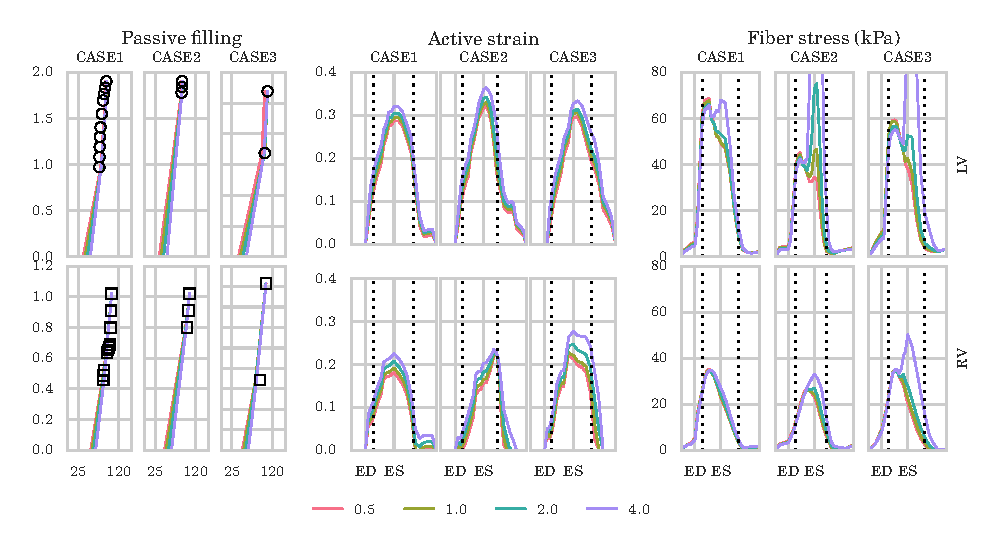
\includegraphics[width=\textwidth]{figures/startsens_results}
  \caption{\label{paper3:fig:startsens}To the left we show the passive
    filling curves, with volume in ml on the $x-$axis and pressure in
    kPa on the $y-$axis with different unloaded volume resulting from
    different material parameters used to estimate the unloaded
    geometries. Middle and right panel show average time traces of
    estimated active strain and Cauchy fiber stress respectively for
    different choice of unloaded configuration. Top row shows the
    results in the left ventricle while bottom row shows the results
    in the right ventricle. Here the values $a = 0.5, 1.0, 2.0$ and
    $4.0$ kPa are used to unload the ventricles. }
\end{figure}



\newpage
\bibliographystyle{plain}
\bibliography{chapters/paper3/bibliography}


